% Oppikirja sivu 411-447
\frame{
\frametitle{Latausjärjestelmä ja energianhallinta}
\begin{itemize}
\item Auton sähköenergian kulutus riippuu varustetasosta ja säätilasta.
\item Sähköenergian kulutus voi olla 1,5 kW tai enemmänkin.
\item Nykyaikaisia autoja ladataan vaihtosähkögeneraattorilla (= "laturilla"), jonka tuottama
sähkö tasasuunnataan diodeilla.
\item Vanhoissa (1970-luku ja vanhemmat) autoissa voi olla tasasähkölaturi. Puolijohdetekniikan kehittyminen
johti tasasähkögeneraattorien korvaamiseen vaihtosähkögeneraattorilla \& tasasuuntaajalla.
\end{itemize}
}

\frame{
\frametitle{Vaihtosähkögeneraattori}
\begin{itemize}
\item Tehokkaimmat generaattorit tuottavat noin 200 ampeerin latausvirran.
\item Tämä vastaa noin 2,8 kilowatin sähkötehoa (14 V x 200 A = 2800 W).
\item Generaattorin toimintajännite on 12 voltin järjestelmässä 14 volttia tai hieman enemmän.
\item Pikkuautoissa pärjätään yleensä 60-80 ampeerin laturilla. Varustemäärän kasvaessa vaaditaan tehokkaampi laturi.
\end{itemize}
}

\frame{
\frametitle{Energian tarve} % Nieminen: auton sähkölaitteet, s.128
\begin{itemize}
\item Pakolliset kuluttajat (sytytys, moottorinohjaus, polttoainepumppu, instrumentit\ldots) kuluttavat noin 200 wattia tehoa.
\item Valot kuluttavat myös 200-300 wattia.
\item Lämmittimet ja puhaltimet kuluttavat yleensä yli 100 wattia kukin.
\item Jos ilmastointijärjestelmän kompressori on sähkökäyttöinen, se kuluttaa tyypillisesti 500-1000 wattia tehoa. Tehokkaammat
kompressorit ovat  hihnavetoisia.
\end{itemize}
}

\frame{
\frametitle{Generaattorin rakenne}
\begin{itemize}
\item Generaattorin rungossa sijaitsee staattorikäämitys, ja pyörivässä roottorissa on roottorikäämitys.
\item Sähköteho otetaan ulos staattorikäämitykseltä. Jännitettä säädetään säätämällä roottori- eli magnetointi- eli kenttävirtaa.
\item Kenttävirta syötetään roottorille liukurenkaiden kautta hiiliharjojen avulla.
\item Kenttävirta (muutama ampeeri) on huomattavasti pienempi kuin staattorilta otettava latausvirta (kymmeniä tai jopa muutama sata ampeeria). 
\end{itemize}
}

\frame{
\frametitle{Generaattorin rakenne}
\begin{itemize}
\item Generaattorista saadaan sitä suurempi taajuus, mitä suurempi on generaattorin {\em napaluku}.
\item Esimerkiksi tuotettaessa 50 Hz sähköä, 2-napainen generaattori tuottaa sitä 3000 rpm pyörintänopeudella,
4-napainen 1500 rpm pyörintänopeudella, 6-napainen 1000 rpm jne..
\item Tyypillisen vaihtovirtalaturin staattorikäämitys koostuu kuudesta käämivyyhdistä, jolloin napaluku on 12.
\item Generaattori on hihnakäyttöinen, ja se pyörii yleensä 2-3 kertaisella nopeudella verrattuna kampiakseliin. Tällainen
välityssuhde varmistaa riittävän pyörimisnopeuden myös tyhjäkäynnillä.
\end{itemize}
}

\frame{
\begin{center}
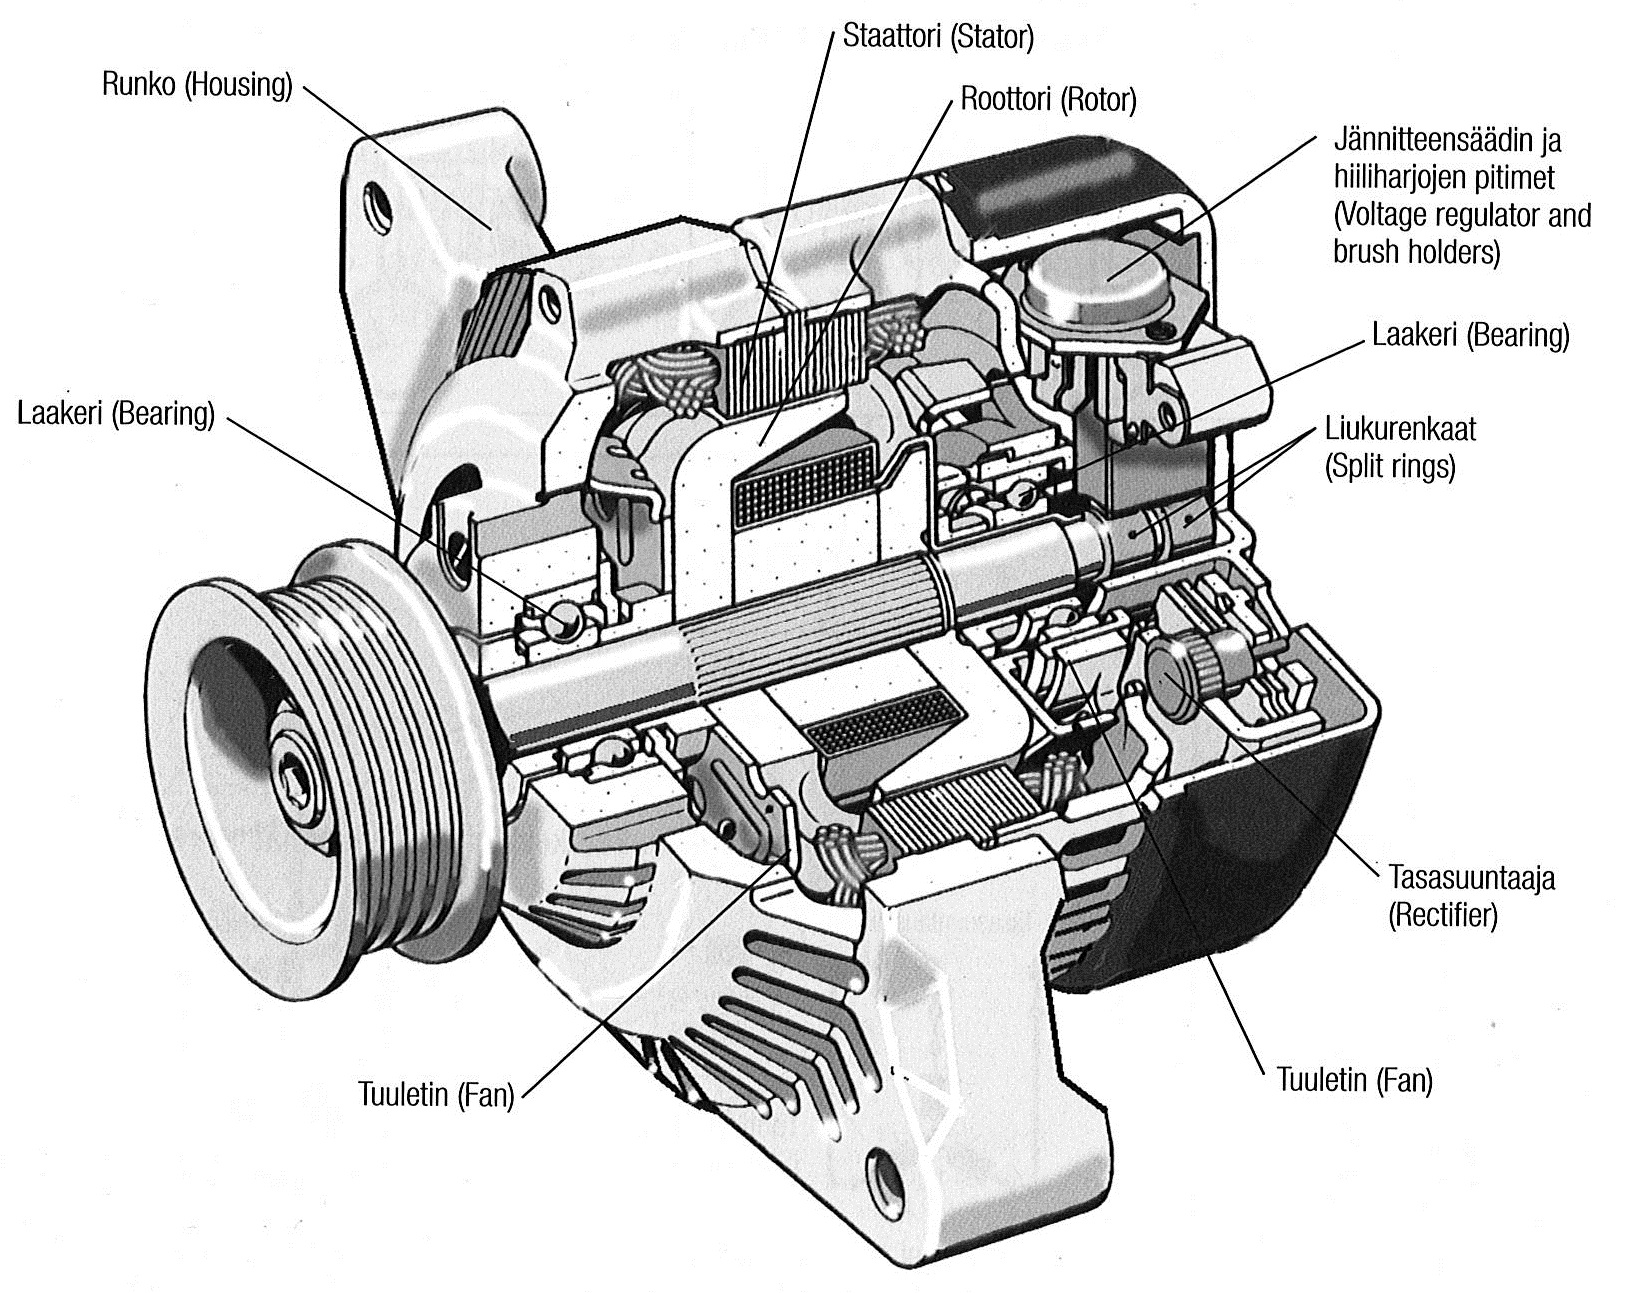
\includegraphics[height=80mm]{latausjarjestelma_pics/laturi.jpg}
\end{center}
\tiny Kuvan lähde: Simo Nieminen: {\em Auton sähkölaitteet}, 1. painos (2008), WSOY, sivu 131.
}

\frame{
\begin{center}
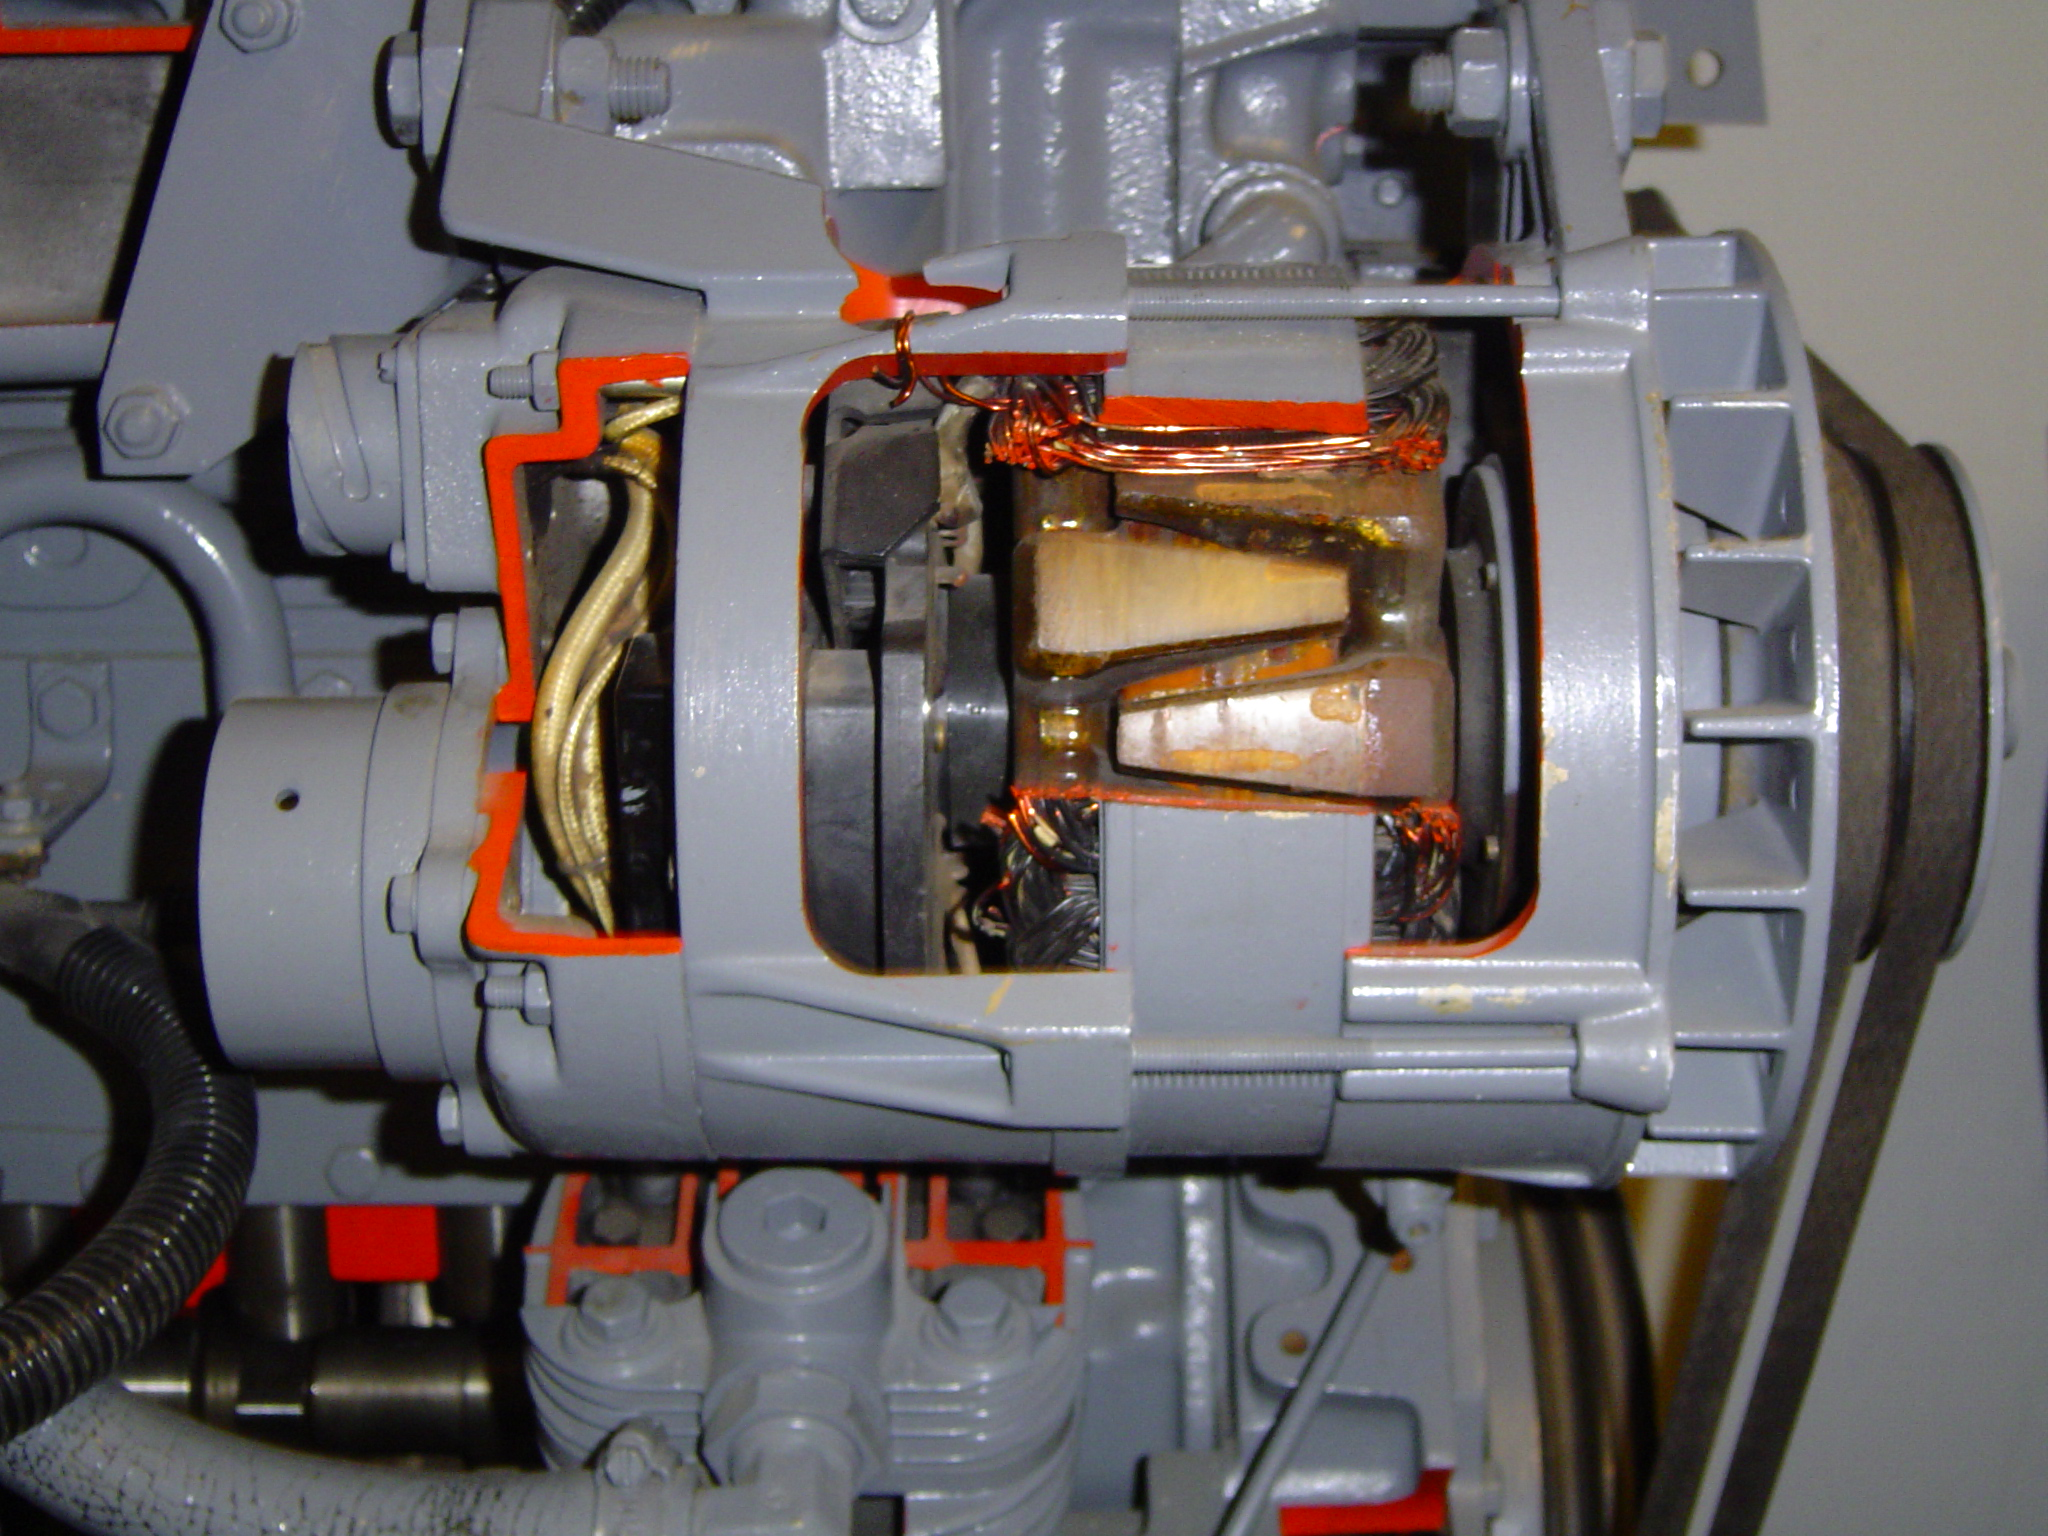
\includegraphics[height=80mm]{latausjarjestelma_pics/dynamo.jpg} % http://en.wikipedia.org/wiki/File:Dynamo.JPG
\end{center}
\tiny \url{http://en.wikipedia.org/wiki/File:Dynamo.JPG}
}

\frame{
\begin{center}
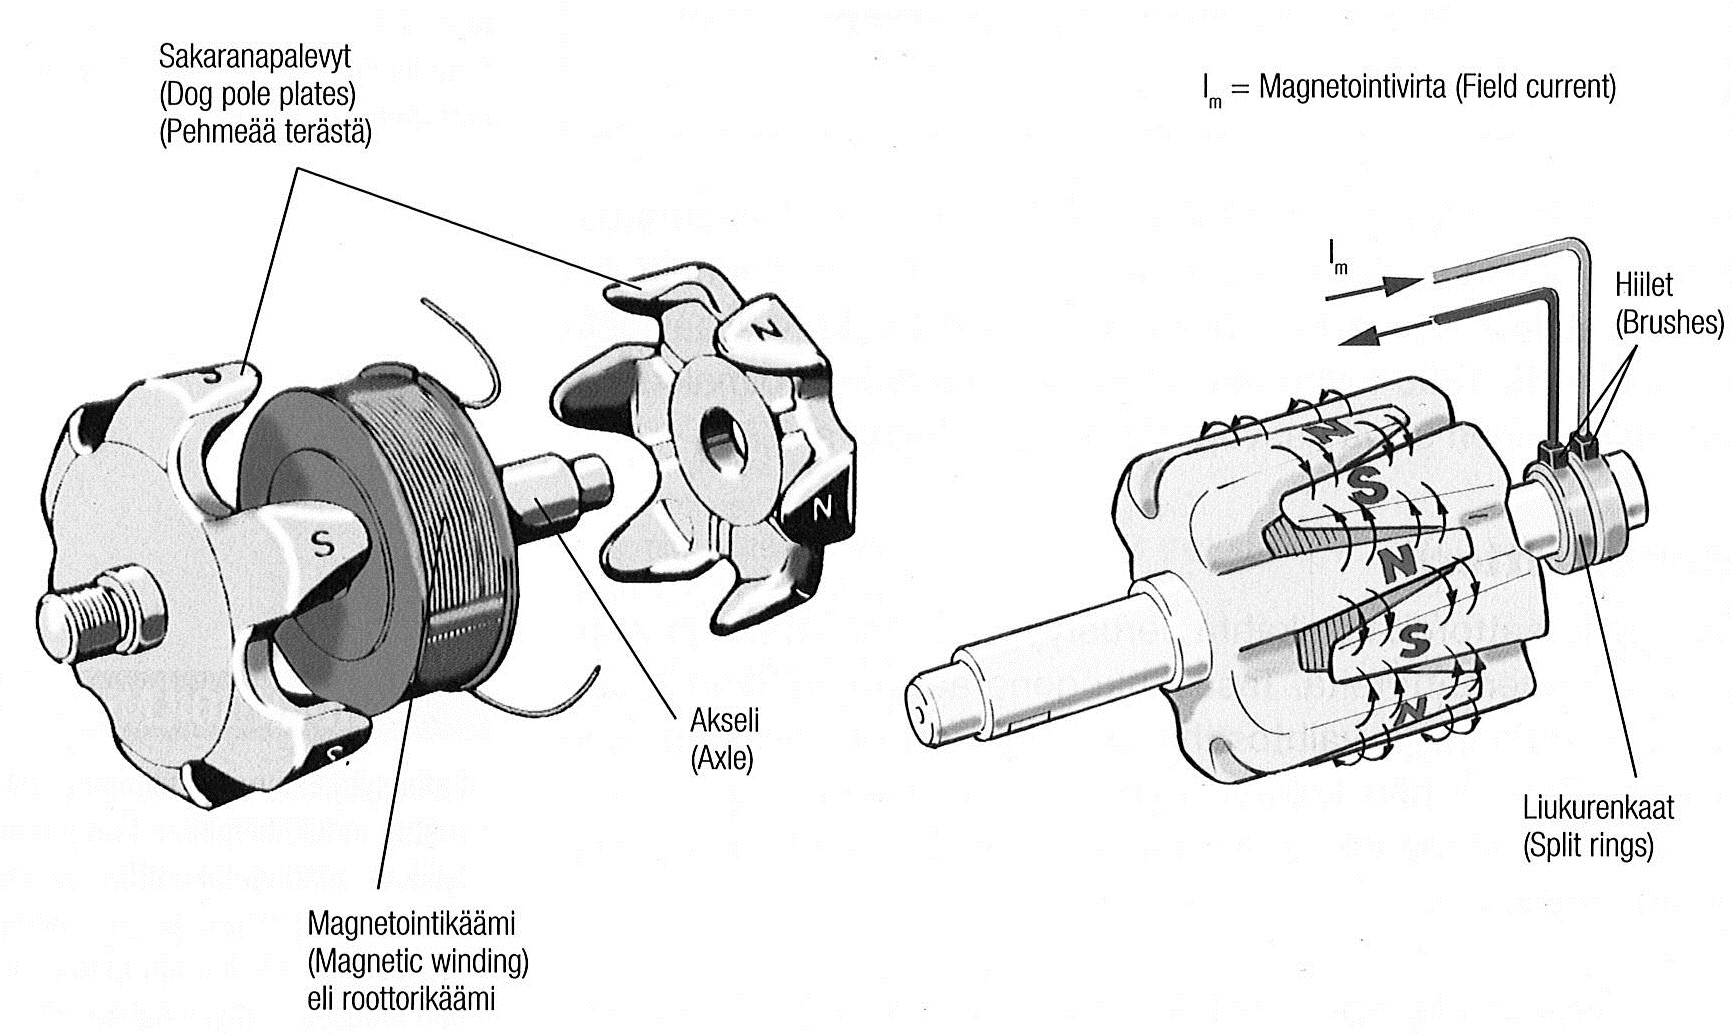
\includegraphics[height=70mm]{latausjarjestelma_pics/roottori.jpg}
\end{center}
\tiny Kuvan lähde: Simo Nieminen: {\em Auton sähkölaitteet}, 1. painos (2008), WSOY, sivu 130.
}

\frame{
\frametitle{Generaattorin rakenne}
\begin{itemize}
\item Roottorin rakenne on erittäin yksinkertainen, joten se ei rikkoudu suurista kierrosnopeuksista.
\item Latausvirta otetaan ulos staattorikäämeiltä. Käämit kytketään joko tähteen tai kolmioon.
\item Käämit on kytketty diodisiltaan, joka tasasuuntaa jännitteen tasajännitteeksi.
\end{itemize}
}

\frame{
\frametitle{Hyötysuhde}
\begin{itemize}
\item Vaihtovirtalaturin (+jännitteensäätimen) hyötysuhde on hieman yli 50 prosenttia.
\item Häviöitä aiheutuu esimerkiksi pyörrevirroista, johtimien resistansseista, kitkasta ja jäähdytyspuhaltimesta. 
\item Suurilla vakionopeudelle optimoiduilla generaattoreilla päästään lähes 100 prosentin hyötysuhteeseen.
\end{itemize}
}

\frame{
\frametitle{Esimerkki nelinapaisesta generaattorista}
\url{http://www.electricalknowledge.com/images/2Phase4poleGeneratorAnimatedDiagramSlow.gif}

}



\frame{
\frametitle{Jännitteensäädin}
\begin{itemize}
\item Periaate sama kuin missä tahansa säätöpiirissä.
\item Jos jännite meinaa nousta yli ohjearvon, kenttävirtaa pienennetään.
\item Jos jännite meinaa laskea alle ohjearvon, kenttävirtaa kasvatetaan.
\end{itemize}
}

\frame{
\frametitle{Jännitteensäädin}
\begin{itemize}
\item Oppikirjan sivulla 419 on esimerkki jännitteensäätimen kytkentäkaaviosta.
\item Uusia jännitteensäätimiä ohjataan usein digitaalisesti. Tämä mahdollistaa useita vikadiagnoositoimintoja, generaattorin
virrantuoton viivyttämisen moottoria käynnistettäessä sekä hidastetun latausvirran muutoksen (ei äkillisiä kuormituspiikkejä hihnalle).
\end{itemize}
}

\frame{
\begin{center}
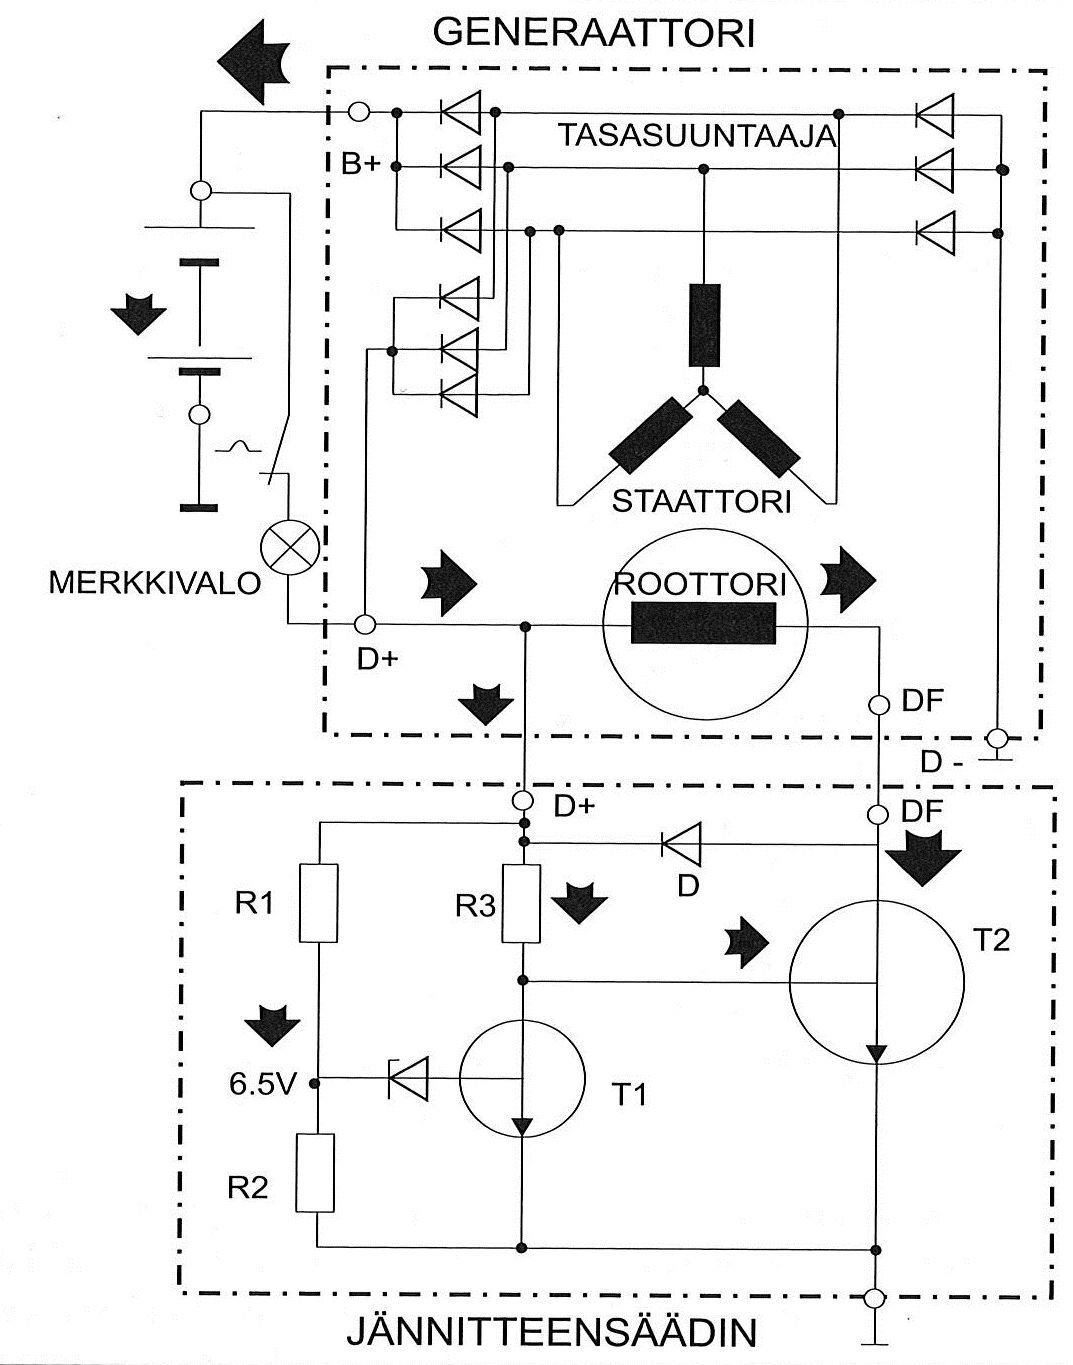
\includegraphics[height=80mm]{latausjarjestelma_pics/saadin.jpg}
\end{center}
\tiny Kuvan lähde: Juhala--Lehtinen--Suominen--Tammi: {\em Moottorialan sähköoppi}, 8. painos (2005), Autoalan koulutuskeskus, sivu 419.
}

\frame{
\frametitle{Mekaaninen jännitteensäädin}
\begin{itemize}
\item Vanhoissa generaattoreissa jännitteensäädin oli mekaaninen säädin, joka katkoi kenttävirtaa sopivasti.
\item Mekaaniset osat kuluvat nopeasti, siksi niistä pyritään eroon suunnittelussa.
\end{itemize}
}

\frame{
\frametitle{Liukurenkaaton generaattori}
\begin{itemize}
\item Generaattorin kuluvin osa on liukurenkaat hiiliharjoineen.
\item Liukurenkaattomassa generaattorissa magnetointikäämi on kytketty staattoriin, ja roottori toimii
ainoastaan magneettivuon ohjaimena.
\item Pienissä työkoneissa ja moottoripyörissä käytetään kestomagneettigeneraattoreita.
\item Kestomagneettigeneraattorin lähtöjännitettä säädetään pulssinleveysmodulaatiolla.
\end{itemize}
}

\frame{
\frametitle{Virranrajoitus}
\begin{itemize}
\item Sähkömagnetismiin perustuvan generaattorin virta rajoittuu luonnostaan johonkin maksimiarvoon, joten
erillistä suojapiiriä ei välttämättä tarvita.
\item Esimerkiksi pyörimisnopeuden kasvu kasvattaa jännitteen taajuutta, jolloin käämien induktanssi rajoittaa virtaa.
\end{itemize}
}

\frame{
\frametitle{Latausjärjestelmän huoltotoimenpiteet}
\begin{itemize}
\item Hihnan kireyden tarkastus.
\item Johtimien kunnon tarkastus.
\item Generaattorin puhdistus.
\item Hiilten vaihto.
\end{itemize}
}

\frame{
\frametitle{Akun varautumisen valvontajärjestelmä}
\begin{itemize}
\item Uusissa autoissa on jännitteensäätimen lisäksi akun varautumisen valvontajärjestelmä, joka seuraa muun muassa akun latausvirtaa. Virtatunnistin sijoitetaan esimerkiksi akkukenkään.
\item Valvontajärjestelmä muun muassa ottaa huomioon akun lämpötilan. Latausjännitettä voidaan nostaa kylmällä säällä reilusti yli 14
voltin, jos auton valot toimivat PWM-säädöllä. Tällöin polttimot eivät rikkoonnu.
\item Järjestelmä seuraa kokonaisvaltaisesti varaustilannetta ja kytkee lisälaitteita tarvittaessa pois päältä, tai nostaa tyhjäkäyntinopeutta.
\end{itemize}
}


\frame{
\frametitle{Vianhaku}
\begin{itemize}
\item Korjausoppaassa on kerrottu ohjearvot latausjärjestelmälle.
\item Latausjännite on tyypillisesti 13,8--14,4 volttia, kun kierrosluku on 2500 rpm.
\end{itemize}
}

\frame{
\frametitle{Vianhaku}
\begin{itemize}
\item Diodien ja käämien kunto on helppo testata yleismittarilla.
\item Yleismittarissa on erityinen dioditestaustoiminto, jolla voi mitata diodin kynnysjännitteen.
\item Kynnysjännite on yleensä 0,6...1 V päästösuuntaan. Estosuuntaan ehjä diodi ei johda.
\item Roottorikäämin resistanssi on yleensä muutamia ohmeja, staattorikäämeillä huomattavasti alle ohmin.
\end{itemize}
}

\frame{
\frametitle{Generaattorin merkinnät}
Bosch-generaattoreissa käytetään merkintöjä
\begin{itemize}
\item Vanha tapa: 14 V 35 A 24: nimellisjännite 14 V, maksimituotto 35 ampeeria ja se pyörintänopeus (2400 rpm), jolla
generaattori tuottaa 3/4 maksimivirrastaan.
\item Uusi tapa: 14 V 23/55 A: nimellisjännite sekä virrantuotot nopeudella 1500 rpm ja 6000 rpm.
\end{itemize}
}
